
\section{Data Mapping Between Meshes}\label{sec:data_mapping_between_meshes}

% introduction, mapping required for operator splitting, different dimensionalities, source to target mesh
% goal is to construct a mapping in the order of the target mesh
% parallel partitioning -> treat source mesh as point cloud

% target->source is interpolation, construct transposed mapping
After the implementation of various solvers for specific parts of the multi-domain model has been described in the previous sections, we now focus on the data mapping between different meshes that occurs in the coupling schemes between the execution of the coupled solvers. 

Data mapping between meshes is required in scenarios that involve both a finely resolved 3D mesh for the electrophysiology model and a coarse 3D mesh for the solid mechanics model. Moreover, data are mapped between the 3D muscle mesh and the embedded 1D fiber meshes in the fiber based electrophysiology model. In these two cases, the mapping has to be carried out in both directions between the involved meshes. The operation can be characterized as \emph{volume mapping}.

We implement a generic mapping scheme between two meshes of any dimensionality and with any relative orientation with respect to each other. 
Given is a finite element interpolant on a \emph{source} mesh, defined by the dof values at the nodes. The goal is to set the dof values of the \emph{target} mesh, such that the error between the finite element representations on the common domain of source and target mesh is as low as possible. By using the ansatz functions of the target mesh, the constructed mapping has the same order of accuracy as the target mesh interpolant. For a linear target mesh, the mapping operation is second order accurate, for a quadratic target mesh, the mapping operation is third order accurate.

The considered source and target meshes are possibly partitioned. In order to perform the data mapping directly between two such meshes without communication between the processes, the partitioning of the volumes would have to be identical. However, this is not practical for different meshes and would disallow different orientations of source and target meshes. The only way to allow such a mapping is to consider either the source or the target mesh as a point cloud and construct the mapping between individual points and a mesh.

Considering the case of mapping the activation parameter value $\gamma$, which is stored on multiple 1D fibers, to the value $\bar{\gamma}$ on the 3D muscle mesh, it is natural to consider the source mesh as a point cloud. Then, instead of multiple fibers, we have a set of points, where $\gamma$ is known. This set of source points is mapped to the enclosing 3D target mesh. On every process, the source points have to be located inside the local subdomain of the target mesh.

The reverse mapping in this example is also required: The geometry of the 3D muscle mesh has to be mapped to the fibers points, such that a deformation of the muscle also affects the embedded fibers. This reverse mapping from the target mesh to the source fiber meshes or points is trivial: The source values can be interpolated in the target mesh using the finite element discretization.
We construct the mapping from source to target mesh to be the transpose operation to this interpolation. In the following section, we introduce the method with a graphical example.

\subsection{Construction of the Parallel Data Mapping}

\Cref{fig:mapping_between_meshes_2} shows a scenario, where data mapping is performed from a source mesh to a target mesh. The source mesh is given by the orange points $s_0$ to $s_3$. The target mesh is visualized by the black and gray elements $e_{\text{T},0}$ to $e_{\text{T},3}$  and nodes $t_0$ to $t_3$.

The value at $s_0$ contributes to all nodes $t_0$ to $t_3$ of the target element $e_{\text{T},0}$ as indicated by the red arrows. The relations between the contributions to $t_0,t_1,t_2$ and $t_3$ are determined by the values of the respective target element ansatz functions $\phi_0$ to $\phi_3$, evaluated at the location of $s_0$.
Similarly, the source points $s_1$ to $s_3$ contribute to the nodes of their enclosing target elements $e_{\text{T},1}$ and $e_{\text{T},2}$. 

% mapping scheme
\begin{figure}%
  \centering%
  \def\svgwidth{0.4\textwidth}
  \input{images/implementation/mapping_between_meshes_2.pdf_tex}%
  \caption{Data mapping scheme from source points (orange) to a target mesh (black).}%
  \label{fig:mapping_between_meshes_2}%
\end{figure}%

As a consequence, all shown source points $s_0$ to $s_3$ influence the value of the target node $t_0$, as indicated by the red arrows.
The value $\hat{t}_0$ at point $t_0$ is computed using the values $\hat{s}_i$ at the points $s_i$ for $i=1,\dots,4$ as follows:
%
\begin{align}\label{eq:mapping_source_target}
  \hat{t}_0 = \s{i=0}{4} \alpha_i\,\hat{s}_i, \quad \text{with }\alpha_i = \dfrac{\phi_{\noexpand\mkern-4mu t_0}(\bfxi_{s_i})}{\s{i=0}{4} \phi_{\noexpand\mkern-4mu t_0}(\bfxi_{s_i})}.
\end{align}
Here, $\phi_{\noexpand\mkern-4mu t_0}$ is the finite element ansatz function for the node $t_0$. It is evaluated at the locations $\bfxi_{s_i}$ of the source points $s_i$ in the respective target elements. The factors $\alpha_i$ specify the fractions, with which the different contributions to $\hat{t}_0$ are scaled. Their construction ensures the property $\sum_{i=1}^4 \alpha_i = 1$.
Note that the number of summands in the sum over the source points can be different from 4 for other target points.

% reverse mapping scheme
\begin{figure}%
  \centering%
  \begin{subfigure}{0.4\textwidth}
    \centering
    \def\svgwidth{\textwidth}
    \input{images/implementation/mapping_between_meshes_3.pdf_tex}%
    \caption{Mapping from target to source points using the reverse scheme of \cref{fig:mapping_between_meshes_2}.}%
    \label{fig:mapping_between_meshes_3}%
  \end{subfigure}
  \quad
  \begin{subfigure}{0.4\textwidth}
    \centering
    \def\svgwidth{\textwidth}
    \input{images/implementation/mapping_between_meshes_4.pdf_tex}%
    \caption{Inverse mapping scheme where the roles of source and target mesh are swapped.}%
    \label{fig:mapping_between_meshes_4}%
  \end{subfigure}
  \caption{Data mapping from target mesh to source mesh.}%
  \label{fig:mapping_between_meshes_34}%
\end{figure}%

The reverse mapping from target nodes to source points uses the same data dependencies between dofs in the source and in the target meshes. \Cref{fig:mapping_between_meshes_3} shows the scheme for the reverse mapping. It is the same as in \cref{fig:mapping_between_meshes_2}, except that the direction of the arrows has been flipped. As noted earlier, the mapping from the target to the source mesh is simply an interpolation in the target mesh. The value $\hat{s}_0$ is computed from $\hat{t}_0$ to $\hat{t}_3$ using the finite element interpolation formula in element $e_{\text{T},0}$:%
\begin{align*}
  \hat{s}_0 = \s{i=0}{4}\hat{t}_i\,\phi_{\noexpand\mkern-4mu t_i}(\bfxi_{s_0}).
\end{align*}
Again, the contribution factors sum up to one, $\sum_{i=0}^4 \phi_{\noexpand\mkern-4mu t_i}(\bfxi_{s_0}) = 1$.

This mapping scheme has the advantage that it requires no communication between the involved processes to determine the target dofs, to which a source dof contributes to. Considering the example in \cref{fig:mapping_between_meshes_2} and assuming that the four target elements are located on four different subdomains, it can be seen that each source point $s_i$ only has to access the target element, where it is contained, to determine the respective element coordinates $\bfxi_{s_i}$.

For the computation of the factors $\alpha_i$ in \cref{eq:mapping_source_target} and for the computation of the target dofs, communication is required. This communication step is the same exchange of ghost dof values, which is also needed for the assembly of finite element stiffness and mass matrices. In the implementation, it is available by the respective functionality of PETSc as described in \cref{sec:oragnization_of_parallel_partitioned_data}.
The reverse mapping from target to source meshes, i.e., the interpolation scheme, works without any communication as all required data are local to the processes.

Instead of reversing the source to target mapping as described, it is often also possible to change the roles of source and target mesh and construct a new mapping in this way. This is only possible, if the two meshes have the same dimensionality, as in the considered example visualizations with two 2D meshes. \Cref{fig:mapping_between_meshes_4} shows the presented mapping scheme with the roles of source and target meshes reversed.
By comparing with \cref{fig:mapping_between_meshes_3}, it can be seen that, in this case, the node $t_0$ contributes to the same nodes $s_0$ to $s_3$ in both approaches. However, the contribution factors are different. In general, the dependent nodes in both meshes are not necessarily the same in the two mapping directions. This means that, in general, the reversed or transposed mapping is not equal to the inverse mapping that is created by interchanging source and target meshes.

For mappings between different dimensionalities, only the approach of reversing the mapping in one direction is possible. For example, mapping from a 1D mesh to a 3D mesh allows no interpolation in the 1D mesh to get the 3D mesh data, as the 1D mesh occupies only a subset of the domain of the 3D mesh. This is a reason for implementing the presented mapping scheme, where the mapping direction can be reversed. Another advantage is that, once the mapping is constructed, both mapping directions are available and the expensive operation of locating the points of one mesh inside the elements of the other mesh has only be performed once.

\subsection{Special Treatment of Coarse Meshes}
% special case with coarse meshes

% reverse mapping scheme
\begin{figure}%
  \centering%
  \begin{subfigure}{0.4\textwidth}
    \centering
    \def\svgwidth{\textwidth}
    \input{images/implementation/mapping_between_meshes_5.pdf_tex}%
    \caption{Mapping scheme from source to target mesh.}%
    \label{fig:mapping_between_meshes_5}%
  \end{subfigure}
  \quad
  \begin{subfigure}{0.4\textwidth}
    \centering
    \def\svgwidth{\textwidth}
    \input{images/implementation/mapping_between_meshes_6.pdf_tex}%
    \caption{Reverse mapping scheme from target mesh to source points.}%
    \label{fig:mapping_between_meshes_6}%
  \end{subfigure}
  \caption{Data mapping scheme with additional data dependencies for a coarse source mesh.}%
  \label{fig:mapping_between_meshes_56}%
\end{figure}%

While the mapping error in the described scheme converges to zero, when the mesh widths approach zero, an issue occurs, if one of the meshes is significantly coarser than the other. \Cref{fig:mapping_between_meshes_5} depicts the case of a coarse source mesh in orange color that is mapped to a finer target mesh in black and gray colors. According to the presented scheme, the source points $s_0$ and $s_3$ contribute to target nodes as visualized by the red arrows. The analog contributions for $s_1$ and $s_2$ are not shown in \cref{fig:mapping_between_meshes_5}. Some target mesh nodes in this example have large distances to the source points and, as a result, do not get contributions from any source point. For example, this is the case for the target points $t_1$ and $t_2$.

To define the value at $t_2$ depending on the source data, we add new contributions from all nodes of the source element in which $t_2$ is located. These contributions are visualized by the yellow arrows in \cref{fig:mapping_between_meshes_5}.
The contributions use the ansatz functions of the source element, and the operation is equivalent to interpolating the value for $t_2$ in the source mesh:
\begin{align*}
  \hat{t}_2 = \s{i=0}{4}\hat{s}_i\,\phi_{\noexpand\mkern-4mu s_i}(\bfxi_{t_2}).
\end{align*}
The location $\bfxi_{t_2}$ of $t_2$ in element coordinates of the source element is required for this computation. Analogously, corresponding contributions are added for the other target nodes that do not yet get any contribution from the source data.

These additional contributions are also present in the reversed mapping scheme from the target to the source mesh. As can be seen in \cref{fig:mapping_between_meshes_6}, the value at $t_2$ contributes to the source nodes $s_0$ to $s_3$. At any source node, the number of contributions increases accordingly. The visualization in \cref{fig:mapping_between_meshes_6} shows five incoming arrows with contributions for $s_0$ and $s_3$. The actual number is higher, since not all target nodes with additional contributions are visualized. At the target nodes, the contribution factors get rescaled, such that they add up to 1 and their relations are preserved.

\subsection{Computation of Element Coordinates For Mapped Points}

During the setup of the mapping between the source mesh and the target mesh, we need to find, for every source point $s_i$, the target element $e_{\text{T},j}$ that contains $s_i$. Furthermore, we need to determine the local element coordinates $\bfx_{s_i} = (\xi_1,\xi_2,\xi_3)^\top$ of the point in this element. To check, if the point is inside a particular element, we compute its coordinates in the element coordinate system. If the coordinates $\bfxi$ are inside the range of $[0,1]^d$, the point is considered inside this element, and the coordinates are determined.

The source point is given by coordinates $\bfx=(x_1,x_2,x_3)^\top \in \R^3$ in the world coordinate frame. The point is related to the $d$-dimensional element coordinate frame $(\xi_1,\dots,\xi_d)$ of its containing target element by the following map:
\begin{align}\label{eq:mapping_parameter_world}
  \bfx(\bfxi) = \s{i=1}{n_\text{dofs}} \phi_i(\bfxi)\, \bfx^i.
\end{align}
Here, $\phi_i$ for $i=1,\dots,n_\text{dofs}$, are the nodal ansatz functions of the target element. The element  has $n_\text{dofs}$ dofs and is given by its node positions $\bfx^i$.

The computation of the element coordinates $\bfxi$ from the world coordinates $\bfx$ consists of inverting the mapping in \cref{eq:mapping_parameter_world}. In the following, several approaches are presented to perform this inversion for different mesh types.

For meshes of type \code{StructuredRegularFixedOfDimension<D>}, the inversion can be performed analytically. The mesh is a Cartesian grid with a fixed mesh width $h$. For quadratic elements, $h$ denotes the side length of an element, not the distance between adjacent nodes.
The computation of the element coordinates $\bfxi$ for the point $\bfx$ uses the position $\bfx^1$ of the first node and is given by:
\begin{align*}
  \bfxi = (\bfx - \bfx^1) / h.
\end{align*}
This formula is also used for 1D meshes of any type.

For non-Cartesian 2D meshes with linear ansatz functions, i.e., meshes of type \code{Struc}\code{tured}\code{DeformableOfDimension<2>}, the inversion of the mapping from element to world coordinate frame in \cref{eq:mapping_parameter_world} can also be done analytically. We consider this problem in a generic way, where both the point $\bfx$ and the nodes $\bfx^1$ to $\bfx^4$ of the 2D element are embedded in 3D space, $\bfx,\bfx^1,\dots,\bfx^4 \in \R^3$. The computation determines the element coordinates $(\xi_1,\xi_2)$ of the projection of $\bfx$ onto the plane of the triangle $(\bfx^1,\bfx^2,\bfx^3)$. 

This functionality is used for specifying electrodes on the skin surface. The electrode positions are specified as a 2D grid in 3D space above the muscle. The mapping automatically projects the points of this grid onto the surface of the 3D mesh. \Cref{fig:electrodes} shows such a use case. A simulation of surface EMG is shown, the coloring corresponds to the potential $\phi_b$ in millivolts in the body domain. A grid of electrode points, visualized by spheres, is mapped onto the surface of the muscle mesh and simulates electrode patches that capture high density surface EMG.

% electrodes
\begin{figure}%
  \centering%
  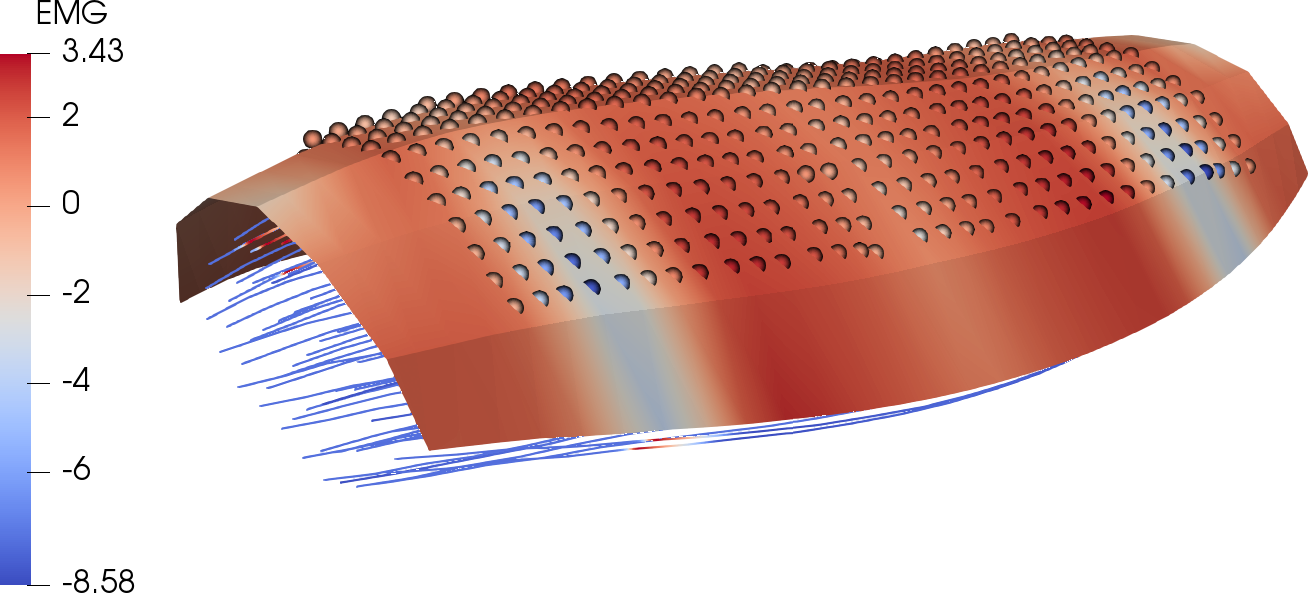
\includegraphics[width=\textwidth]{images/implementation/electrodes.png}%
  \caption{Simulation of surface EMG using the fiber based electrophysiology model with body fat layer. Only the top surface of the fat layer mesh is shown. The spheres correspond to the position of surface electrodes that are used to sample the simulation result in a spatial grid.}%
  \label{fig:electrodes}%
\end{figure}%

After calculating the mentioned projection on the 2D plane, the computation has to invert the map in \cref{eq:mapping_parameter_world}. The ansatz functions $\phi_i$ are bilinear in the coordinates $\xi_1$ and $\xi_2$. This quadratic equation has two solutions for the unknown coordinates $\bfxi$. The formulas for those solutions have been determined using the symbolic mathematics toolbox \emph{SymPy} \cite{meurer2017sympy} and the solution, where the point is inside the element or closer to its center is chosen.

For generic hexahedral 3D meshes, \cref{eq:mapping_parameter_world} is a cubic equation in $\bfxi$, and the analytic inversion is not feasible. However, for simplex elements, i.e., tetrahedra given by points $\bfx^1$ to $\bfx^4$, it is possible. The ansatz in this case is given by:
\begin{align*}
  \bfx &= (1-\xi_1-\xi_2-\xi_3)\,\bfx^1 + \xi_1\,\bfx^2 + \xi_2\,\bfx^3 + \xi_3\,\bfx^4.
\end{align*}
This can be reformulated as:
\begin{align}\label{eq:simplex_ansatz}
   \bfx-\bfx^1 &= (\bfx^2 - \bfx^1)\,\xi_1 + (\bfx^3  - \bfx^1)\,\xi_2 + (\bfx^4 - \bfx^1)\,\xi_3.
\end{align}
This linear system of three equations can be solved for the three unknowns $\xi_1,\xi_2$ and $\xi_3$.

To invert the mapping for hexahedral elements, we proceed as follows.
A hexahedral element can be subdivided into five simplex elements. 
Four outer simplex elements share their faces with parts of the hexahedral's surface. One interior simplex element only touches the hexahedron surface by its edges. 

In each of the four outer simplex elements, we define a coordinate system $(\xi_1,\xi_2,\xi_3)$ with the origin located at a corner of the hexahedron. 
In these elements, the coordinates $\bfxi$ for the point $\bfx$ can be computed  using the ansatz in \cref{eq:simplex_ansatz}. The computed coordinate values can be transformed to the hexahedral coordinate system by applying the appropriate mirror operations $\xi \mapsto (1-\xi)$ on some coordinates. Using the average values of the hexahedral coordinates resulting from all four outer simplex elements gives a good approximation for the correct hexahedral element coordinates $\bfxi$ of the point $\bfx$.

To obtain the correct element coordinates, these approximate values are used as initial guess in a Newton scheme, which subsequently tries to find the root of $\bfr = (\bfxi - \bfx(\bfxi))$ and, thus, invert the mapping in \cref{eq:mapping_parameter_world}. 

Runtime measurements have shown that the lower number of Newton iterations resulting from the heuristic with the four simplex elements to compute an initial guess outweighs the additional runtime for the heuristic and, in total, leads to a faster computation.

The Newton scheme uses the inverse Jacobian matrix of the mapping in \cref{eq:mapping_parameter_world}. If the residual norm $\Vert\bfr\Vert_2$ cannot not be brought under the threshold of \num{1e-8} in 16 iterations, this indicates that the problem of inverting the Jacobian is badly conditioned and the Jacobian has a large numerical error. In this case, the optimization is restarted using the derivative-free Nelder-Mead algorithm.

Before applying the Newton and Nelder-Mead algorithms, our implementation performs two basic checks that can directly terminate the computation of the coordinates: First, the coordinates of the point $\bfx$ are compared with the bounding box of all nodes of the element. If the point is outside the bounding box, the element coordinates do not have to be computed, and a different element, which contains the point $\bfx$, is searched. Second, all node positions are checked for equality with the point $\bfx$. If $\bfx$ is the same as one of the node positions, the element coordinates are directly known. This case frequently occurs, if one of source and target mesh is a subset of the other.

\subsection{Conditioning of the Problem and Mapping Tolerances}

As mentioned in the last section, the Newton scheme that solves the inverse problem of mapping a point from elemental coordinates to world coordinates uses the inverse Jacobian matrix of the mapping. The inversion of this matrix has a high numerical error, if the condition number of the Jacobian matrix is large. A large condition number can be found for 3D hexahedral elements, where the two element coordinate directions for $\xi_1$ and $\xi_2$ are almost linearly dependent. This is the case for elements with an interior angle of nearly \SI{180}{\degree}. \Cref{fig:bad_element} shows such an element, which occurs at the outer boundary of the muscle mesh.

% bad_element
\begin{figure}%
  \centering%
  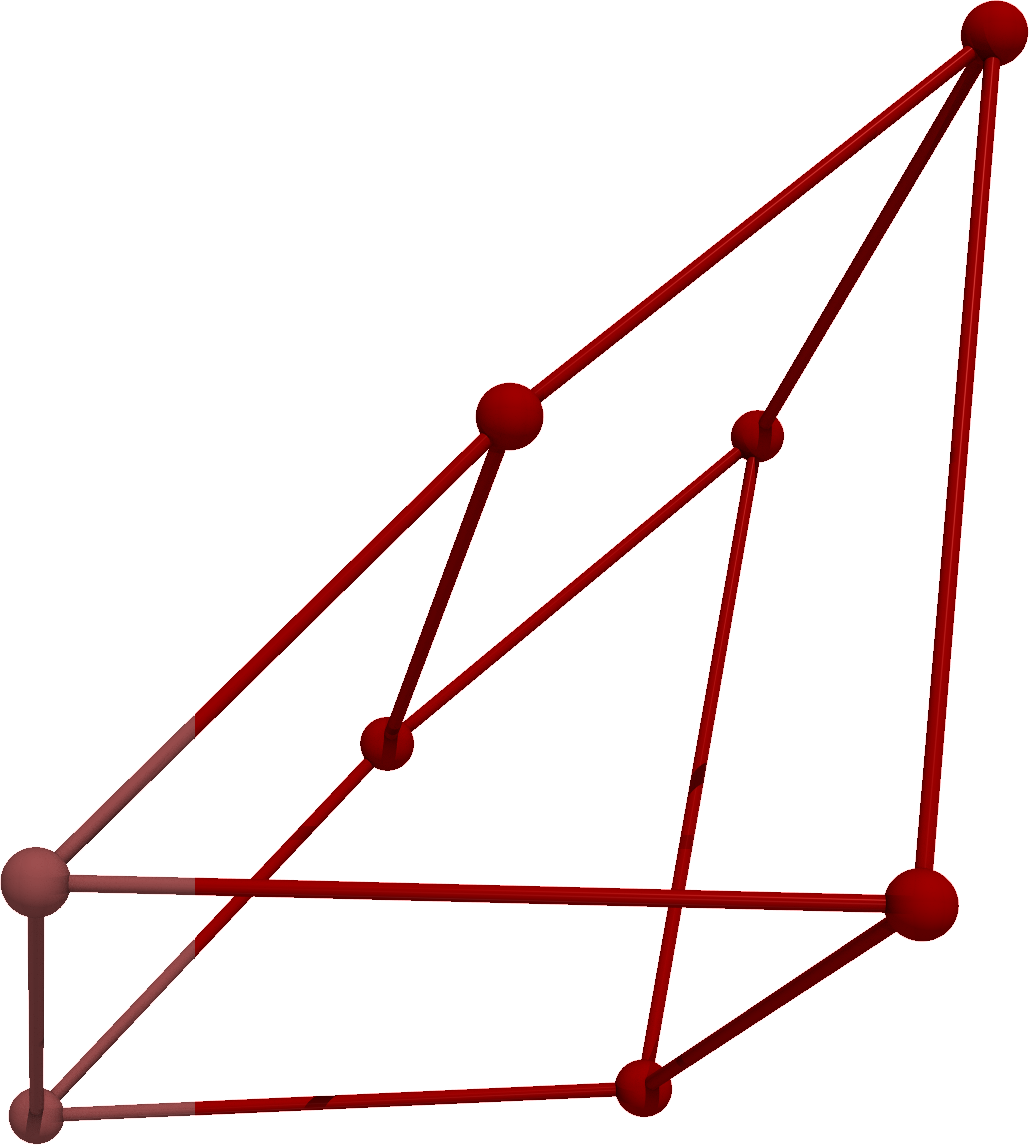
\includegraphics[width=0.3\textwidth]{images/implementation/bad_element2.png}%
  \caption{Hexahedral element of the muscle mesh with an interior angle of nearly \SI{180}{\degree}. Such elements lead to poor conditioning of the Jacobian matrix inversion problem and, as a consequence, require numerous Newton iterations in the setup of the data mapping between meshes.}%
  \label{fig:bad_element}%
\end{figure}%

If the conditioning is too bad and the computed inverse Jacobian has a large numerical error, the Newton scheme fails to find a solution in the given maximum number of iterations and the Nelder-Mead algorithm is used instead. This algorithm usually succeeds. However, it requires significantly more compute time than the Newton scheme. The case where the Nelder-Mead algorithm is needed, however, only occurs for a small number of elements and only in highly-resolved meshes.

\Cref{fig:condition_number2} shows the condition number of the Jacobian matrix of the mapping from element to world coordinates per element. The condition number is numerically approximated using the \emph{von Mises} power iteration algorithm to obtain the largest eigenvalue of the Jacobian and its inverse.
It can be seen in \cref{fig:condition_number7x7} that the elements with the highest condition number are located along longitudinal lines on the outer surface of the muscle mesh. Two such lines exist on both sides of the muscle. The cross-sectional mesh at the top of the muscle shows that the elements along these lines have large interior angles at the respective positions. 

% condition number 7x7
\begin{figure}%
  \centering%
  \begin{subfigure}{0.9\textwidth}
    \centering
    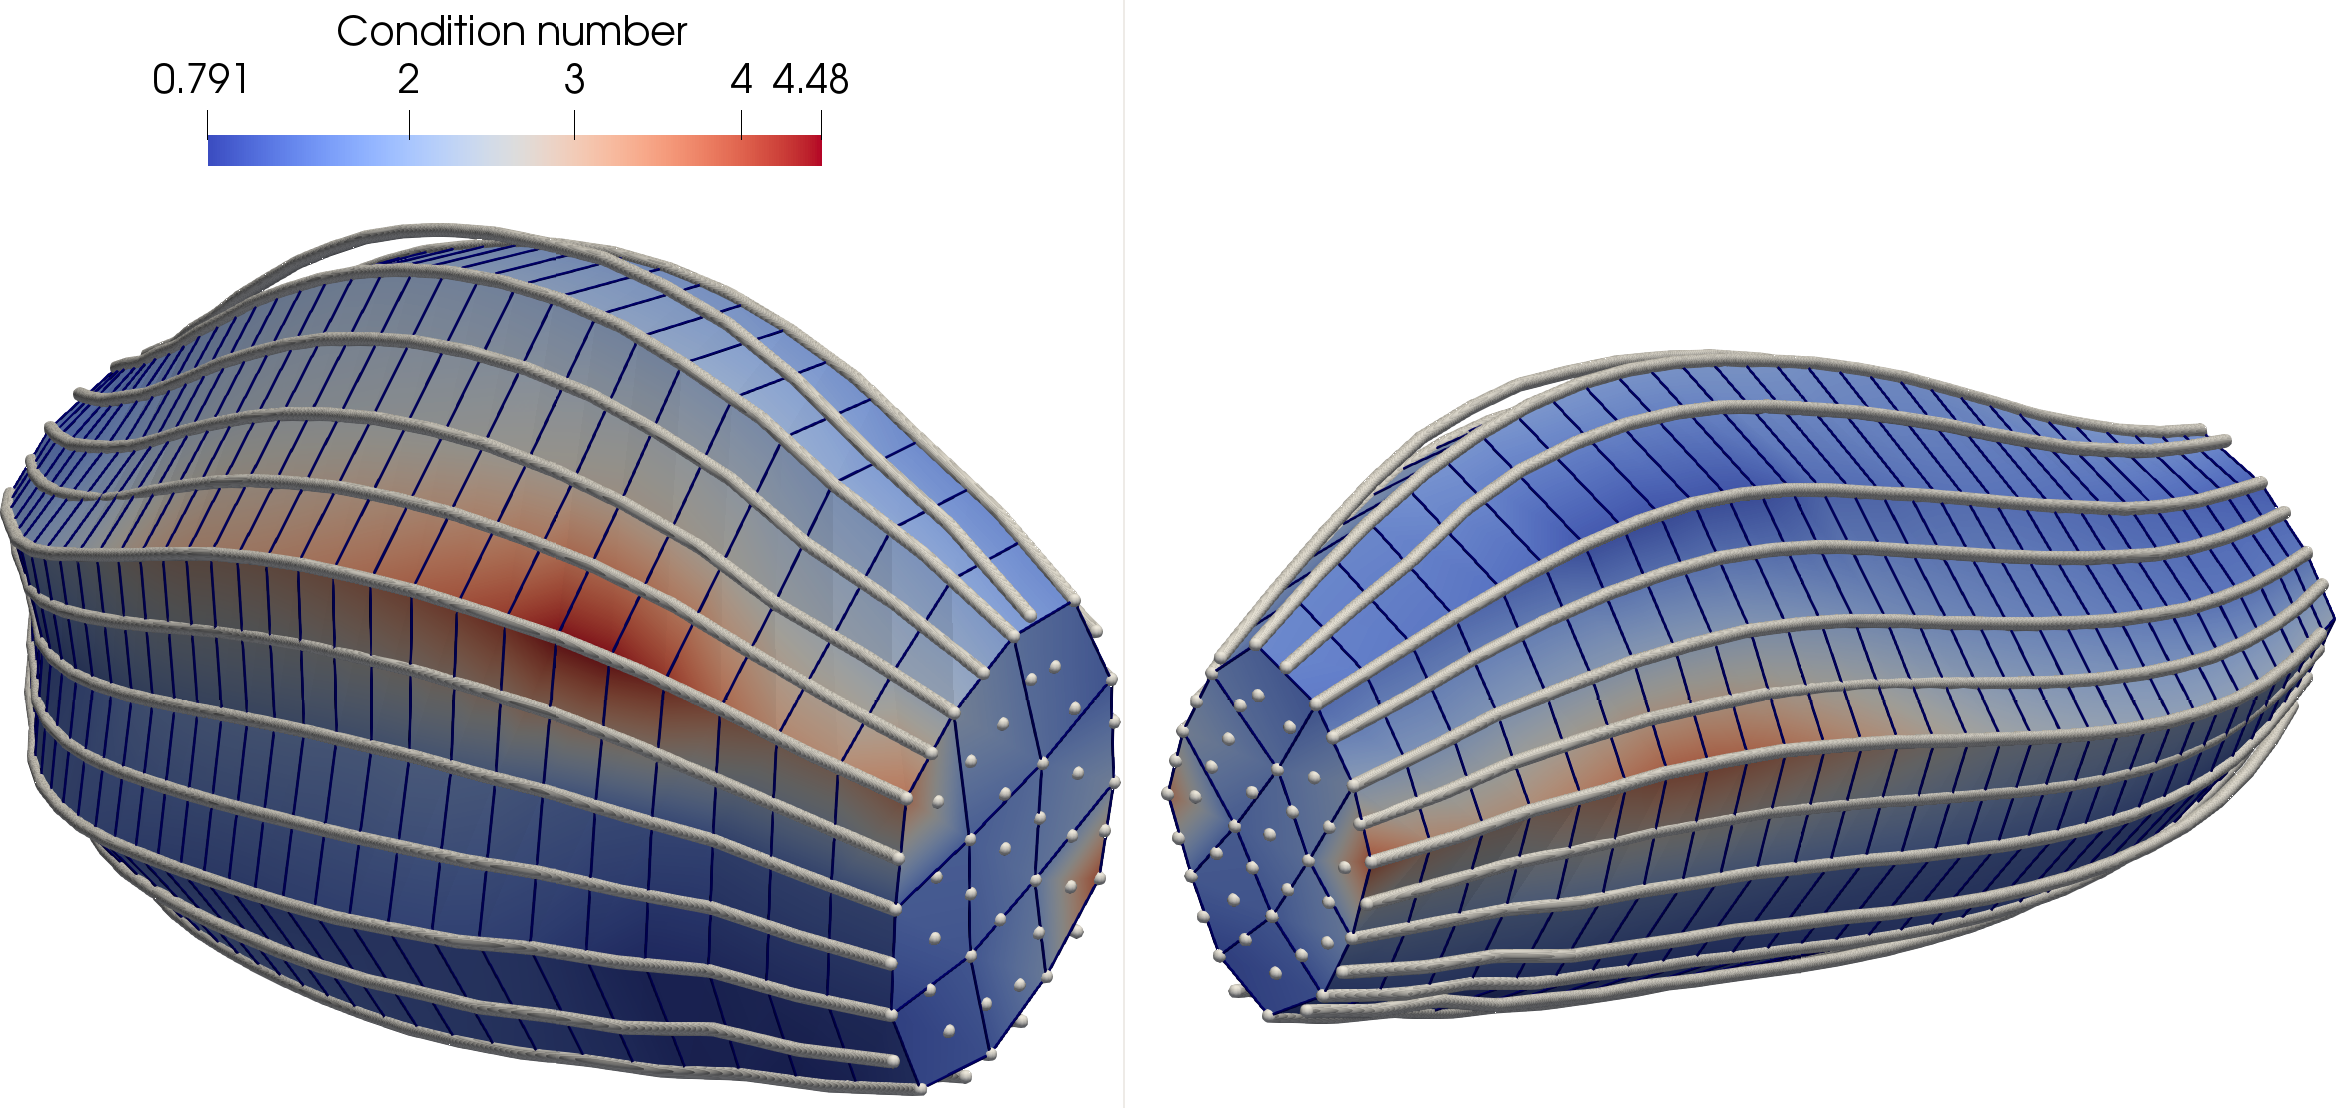
\includegraphics[width=\textwidth]{images/implementation/condition_number.png}%
    \caption{Scenario with $7\times 7$ fibers.}%
    \label{fig:condition_number7x7}%
  \end{subfigure}\\[4mm]
  \begin{subfigure}{0.9\textwidth}
    \centering
    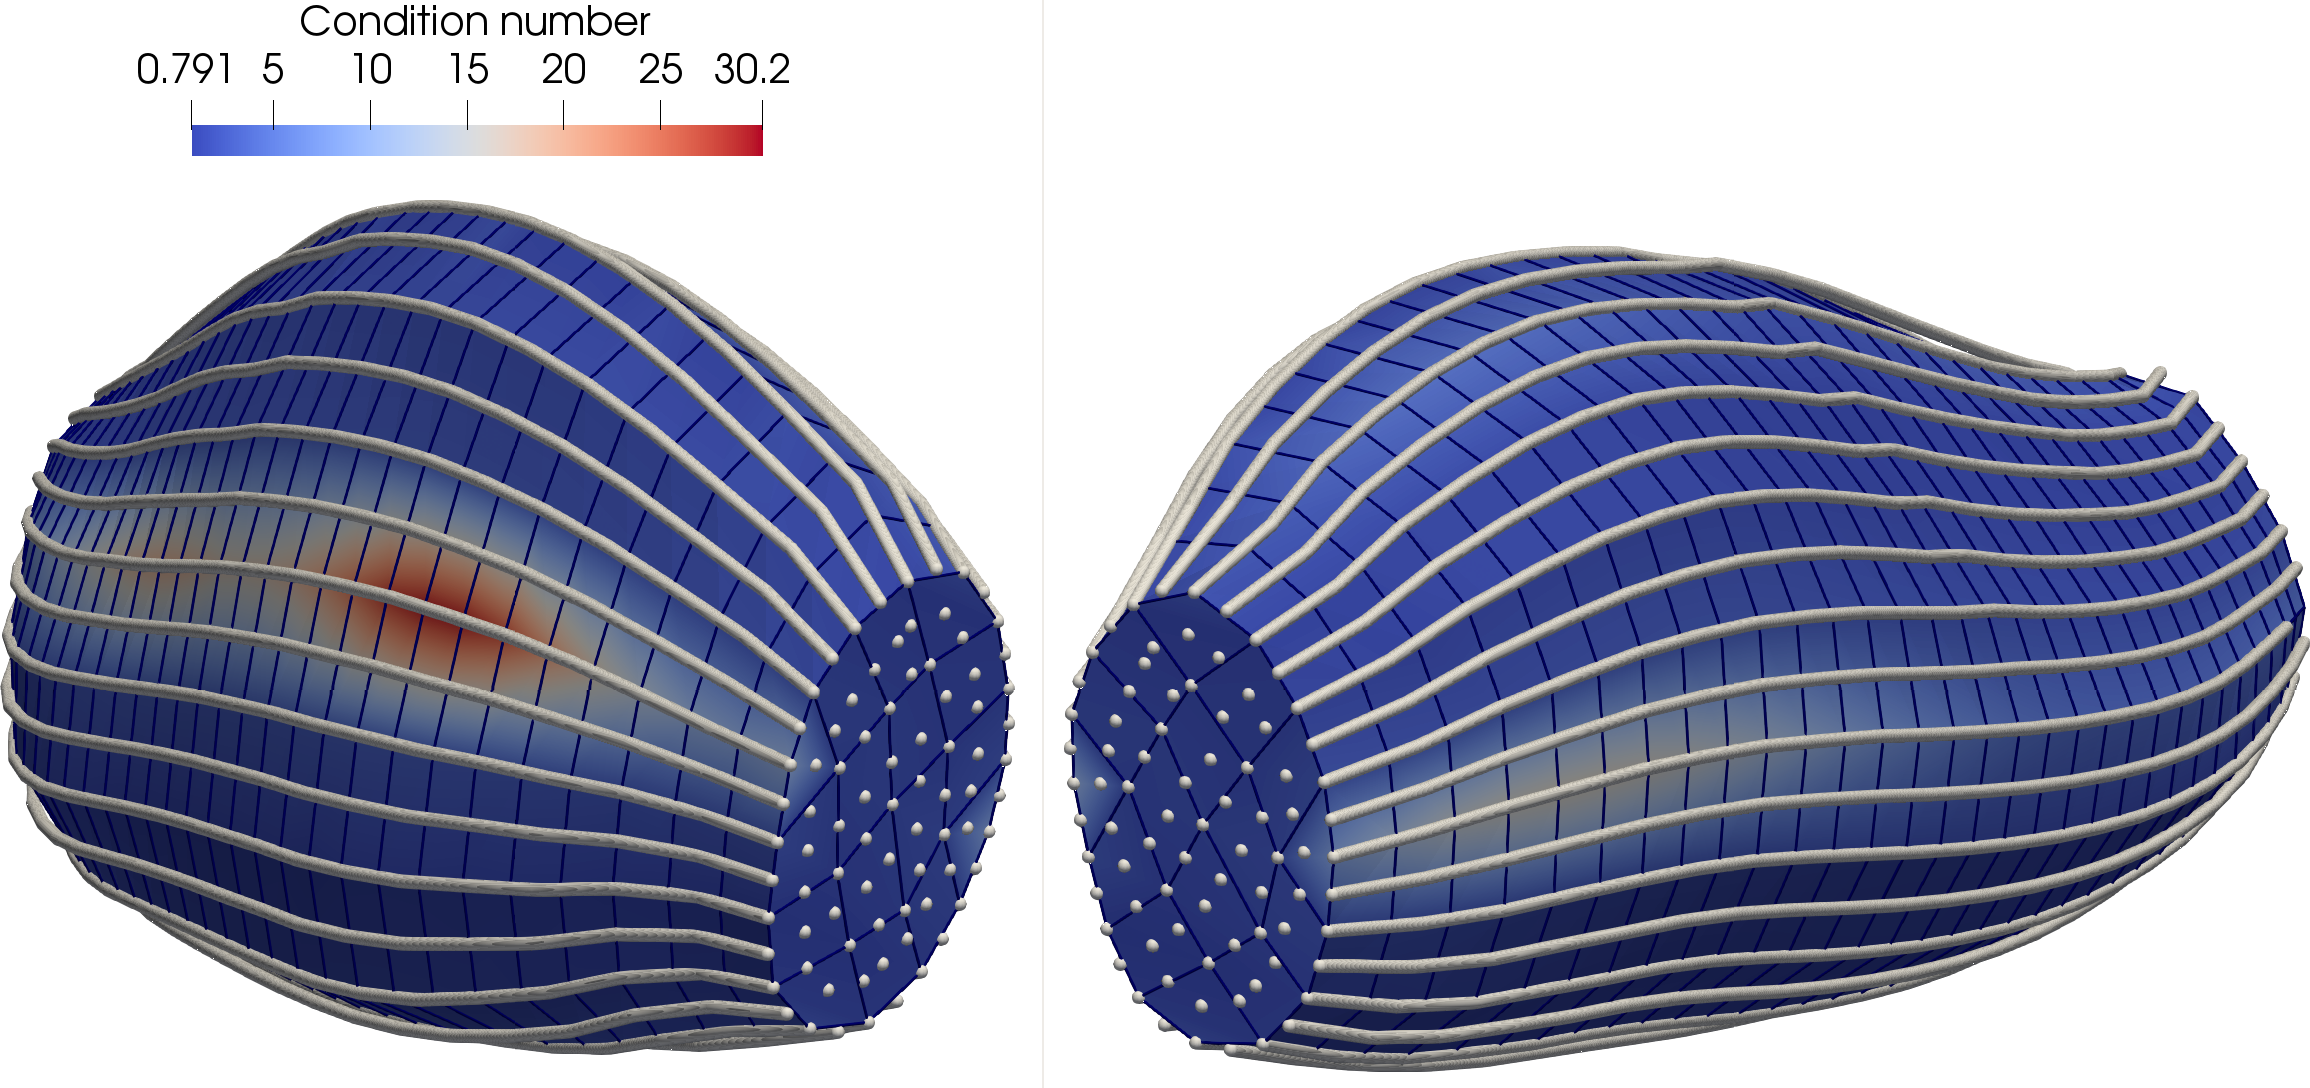
\includegraphics[width=\textwidth]{images/implementation/condition_number2.png}%
    \caption{Scenario with $9\times 9$ fibers}%
    \label{fig:condition_number9x9}%
  \end{subfigure}
  \caption{Fiber meshes and corresponding muscle mesh, obtained with a sampling stride of two. The left and right view show both sides of the muscle mesh. The 3D mesh is colored by the condition number of the Jacobian matrix.}%
  \label{fig:condition_number2}%
\end{figure}%

\Cref{fig:condition_number9x9} shows the same information for a different mesh with $9\times 9$ fibers instead of the subset of $7\times 7$ fibers in \cref{fig:condition_number7x7}. In \cref{fig:condition_number9x9}, the outer surface of the muscle mesh is smoother and the interior angle of the elements along the respective longitudinal lines is even closer to \SI{180}{\degree}. Thus, the resulting maximum condition number has a higher value of \num{30.2} compared to \num{4.48} in the example of \cref{fig:condition_number7x7}.

Another effect can be seen in the visualization in \cref{fig:condition_number7x7}. The muscle mesh was generated from the fiber data with sampling strides of two in the cross-sectional directions. As a consequence, the nodes of the 3D mesh are part of every second fiber. This results in some outer fibers being located outside the domain of the 3D mesh. Such a case can be seen for the upper-most fiber in \cref{fig:condition_number7x7}. 

To also involve such fibers in the computation, we enable data mapping between the 3D mesh and fibers that are outside but close to the 3D mesh. We add a tolerance parameter $\xi_\text{tolerance}$ to the implementation that specifies, how far outside the mesh fibers can be located to still be included in the mapping. On the element level, a point is considered to be part of an element, if its element coordinates $(\xi_1,\xi_2,\xi_3)$ are no further than $\xi_\text{tolerance}$ off the element domain, i.e., for %
\begin{align*}
  -\xi_\text{tolerance} \leq \xi_i \leq 1 + \xi_\text{tolerance}\quad \forall i \in \{1,2,3\}.
\end{align*}
This treats the outside fibers as if they were located inside the 3D mesh. For the fibers in the interior, the threshold leads to potentially multiple neighboring elements claiming ownership of a point. In this case, the element that contains the point without this tolerance value is chosen.
By default, the tolerance value is set to $\xi_\text{tolerance}=0.1$, but it can be adjusted to different values in the Python settings file if needed.

In summary, OpenDiHu can map data between any two overlapping meshes. The inversion of the mapping from elemental to world coordinates is an important task of this problem, which is non-trivial for 3D hexahedral elements and is solved numerically. The combination of fiber meshes with a 3D muscle mesh leads to specific effects such as degraded condition numbers or fibers outside the 3D mesh that have to be considered in the mapping.

\begin{reproduce_no_break}
  The visualizations in \cref{fig:condition_number2} were obtained using the \code{electrophysiology/fibers/fibers_emg} example. The condition number of the Jacobian is computed by the \code{StaticBidomainSolver} if the parameter \code{`enableJacobianConditionNumber`} is set to \code{True}.
\end{reproduce_no_break}
